\chapter{확률, 정보, 엔트로피}

\lectureoverview{통계역학은 미시적 법칙과 불완전한 지식이 만나는 지점에서 시작한다. 먼저 확률을 엄밀하게 정의한 다음, 결정론적 운동 자체가 어떻게 확률을 부여하는지, 보존 법칙이 상태 공간을 어떻게 나누는지, 그리고 정보를 보존하는 동역학이 왜 자연스럽게 엔트로피로 이어지는지 묻는다. 이러한 구조를 갖춘 뒤에야 첫째 법칙과 영 법칙을 다룬다.}

\section{왜 통계역학인가?}

통계역학은 때때로 오래된 물리학으로 묘사된다. 그런 묘사는 핵심을 놓친다. 통계역학은 전근대적이면서 현대적이고, 우리가 아는 이론들을 계승할 탈근대 물리학에서도 유용할 가능성이 크다. 구체적인 모형들은 생겼다가 사라지지만, 열역학 제2법칙은 길잡이로서 거듭 살아남았다. 자연에 대한 어떤 설명이 대가 없이 질서를 만들어 내거나, 근본적으로 정보를 지워 버리거나, 닫힌계를 부자연스러울 만큼 단순한 상태로 몰고 가는 듯 보일 때마다 제2법칙은 빠뜨린 것이 있음을 경고한다.

이 분야는 새로 발견된 입자보다 덜 매력적으로 보일 수 있지만, 적어도 그만큼 깊고 훨씬 더 일반적이다. 기체, 액체, 고체, 복사, 블랙홀, 정보, 양자장 모두 통계적 추론을 필요로 한다. 실제로 입자를 발견하는 데 쓰이는 실험 장비도 통계역학 없이는 이해할 수 없다. 그래서 여러 세대의 뛰어난 물리학자들은 주된 연구 분야가 다른 곳에 있더라도 통계역학을 익혔다. 이 분야는 유용할 뿐 아니라 유난히 아름답기도 하다.

통계역학이 왜 필요한지 보려면 역학이 제시하는 이상적인 상황에서 시작하자. 닫힌계란 고려 대상인 우주 전체이거나, 주변 환경의 영향을 받지 않을 만큼 충분히 고립된 부분계다. 초기 조건과 시간에 따른 변화 법칙을 알면 고전역학은 완전한 예측을 제시한다. 양자역학은 예측할 수 있는 것을 수정하지만, 양자역학 역시 엄밀히 정의된 상태와 이론이 허용하는 최대 정보를 예측하는 법칙을 갖는다.

원리적으로 가능한 예측과 유용한 이해 사이에는 큰 차이가 있다. 이 방에 있는 모든 분자의 위치와 속도를 나열하면 그 목록은 엄청나게 길고 거의 즉시 바뀌며, 우리가 실제로 궁금해하는 질문에는 거의 답하지 못한다. 따라서 정확한 미시적 법칙은 완벽한 예측력을 갖고도 실용적으로는 쓸모없을 수 있다.

통계역학은 이런 물리적 상황에 확률론을 적용하는 분야다. 초기 조건을 완벽한 정확도로 알지 못하거나, 법칙을 근사적으로만 알고 있거나, 계가 열린계이거나, 단순히 미시적 변수의 수가 너무 많아 추적할 수 없을 때 통계역학이 필요하다. 그렇다고 예측이 약해지는 것은 아니다. 많은 경우 큰 수 덕분에 통계적 예측은 놀라울 정도로 정밀해진다.

고립된 기체 상자를 생각해 보자. 모든 분자의 궤적을 예측할 수는 없지만, 몇 가지 거시적 자료만으로도 압력, 에너지와 여러 다른 거시량을 높은 정밀도로 예측할 수 있다. 불확실성이 남는 것은 요동이다. 예측할 수 없는 어느 순간에는 작은 영역에 평균보다 많은 분자가 들어 있고, 다른 영역에는 더 적을 수 있다. 이런 사건은 확률분포의 꼬리 부분에 해당한다. 일어날 가능성은 작지만 금지된 것은 아니다. 특정 사건이 언제 일어날지는 예측하지 못해도, 이런 요동이 얼마나 자주 일어날지는 계산할 수 있다.

동전 던지기에서도 같은 구분을 볼 수 있다. 공정한 동전을 십억 번 던지면 앞면과 뒷면의 횟수는 서로 비슷할 것이다. 충분히 많이 던지다 보면 앞면이 길게 이어지는 경우도 언젠가는 나오지만, 확률론은 그 시점을 미리 정해 주는 대신 그런 연속이 얼마나 자주 일어나는지를 예측한다. 통계역학은 구성 요소가 너무 작거나 너무 많거나 둘 다인 계를 다루기 위해 만들어졌다.

이 강의에서는 물질에 관한 응용뿐 아니라 그 법칙들도 살펴본다. 이 분야는 반복해서 공부할 만한 가치가 있다. 배우고, 일부를 잊고, 다시 배우면서 어떤 생각이 근본적인지 더 깊이 알게 된다. 이후의 모든 내용을 좌우하는 생각부터 시작하자.

\section{원초적 언어로서의 확률}

확률이 왜 작동하는지는 확률 계산 자체가 설명해 주지 않는다. 확률적 예측은 특정 시행에서 빗나갈 수 있다. 결과가 가능하지만 일어날 가능성은 작다는 말이 바로 그런 뜻이다. 확률론은 예외가 어떻게 분포하는지는 알려 주지만, 예외를 없애지는 않는다. 그러므로 확률을 원초적 개념으로 받아들이고, 확률이 따르는 규칙을 제시한다.

\subsection{상태와 정규화}

\(i\)는 계의 가능한 결과나 가능한 상태를 나타낸다고 하자. 동전 하나에서는 \(i\)가 앞면이나 뒷면을 뜻할 수 있다. 주사위 하나에서는 \(1\)부터 \(6\)까지의 값을 가질 수 있다. 주사위 두 개에서는 두 면을 모두 기록하도록 지표 한 쌍을 쓴다. 먼저 유한한 이산 상태공간을 다룬다.
\begin{equation}
 i=1,\ldots,N,
\end{equation}
이후에는 무한히 많은 상태와 연속적으로 변하는 상태로 넘어간다.

무지하다는 것은 계에 상태가 없다는 뜻이 아니다. 계가 어떤 상태에 있는지 모른다는 뜻이므로, 각 가능성에 확률 \(p_i\)를 부여한다. 기본 규칙은 다음과 같다.
\begin{align}
 p_i &\geq 0, \label{eq:sm1-prob-positive}\\
 \sum_{i=1}^{N}p_i &=1. \label{eq:sm1-prob-normalization}
\end{align}
각 대안은 서로 배타적이고 전체를 빠짐없이 포괄한다. 즉, 그중 정확히 하나가 일어난다. 여기서 음의 확률은 의미가 없으며, 허용된 결과 중 하나는 반드시 일어나므로 확률의 합은 1이다.

\subsection{빈도와 대수의 법칙}

확률은 반복 시행을 통해 실험과 연결된다. 같은 실험을 \(N_{\mathrm{trials}}\)번 수행하고, 결과 \(i\)가 나온 시행의 횟수를 \(N(i)\)라고 하자. 그러면 빈도 해석은 다음과 같다.
\begin{equation}
 p_i=
 \lim_{N_{\mathrm{trials}}\to\infty}
 \frac{N(i)}{N_{\mathrm{trials}}}.
 \label{eq:sm1-frequency}
\end{equation}
이는 이상적인 극한을 통해 표현한 물리적 가설이다. 실험실에서 실험을 무한히 많이 수행하는 일은 없다. 충분히 많은 시행을 하면 그 비율이 의도한 예측에 충분히 가까운 \(p_i\)에 이른다는 뜻이다. 유한한 표본에서는 극한값 주변으로 요동이 생긴다.

\subsection{평균}

이제 각 상태에 수 \(f(i)\)를 대응시키자. 이 수는 에너지, 운동량 또는 측정하고자 하는 다른 물리량일 수 있다. 그 기댓값은 다음과 같다.
\begin{equation}
 \langle f\rangle=\sum_i f(i)p_i.
 \label{eq:sm1-expectation}
\end{equation}
대괄호 표기는 양자역학이 아닌 경우에도 편리하다. 빈도로 표현하면 같은 평균은 다음과 같다.
\begin{equation}
 \langle f\rangle
 =
 \lim_{N_{\mathrm{trials}}\to\infty}
 \frac{1}{N_{\mathrm{trials}}}
 \sum_i f(i)N(i).
 \label{eq:sm1-frequency-average}
\end{equation}

동전에 대해 다음과 같이 정의하자.
\begin{equation}
 f(\mathrm{H})=+1,
 \qquad
 f(\mathrm{T})=-1.
\end{equation}
앞면과 뒷면의 확률이 각각 \(1/2\)이면,
\begin{equation}
 \langle f\rangle
 =(+1)\frac12+(-1)\frac12=0.
\end{equation}
평균이 가능한 결과 중 하나일 필요는 없다. 동전은 0에 멈추지 않는다. 0은 동전이 가질 수 있는 두 값의 분포를 요약한다.

이 짧은 설명에서는 이 분야 전반에 쓰일 용어, 즉 상태, 확률, 빈도, 기댓값을 정리했다.

\section{확률을 부여하는 세 가지 방법}

\subsection{대칭성}

동전의 두 면에 보통 같은 확률을 부여하는 이유는 무엇일까? 첫 번째 답은 대칭성이다. 거의 이상적인 동전을 뒤집으면 실험 조건을 바꾸지 않은 채 앞면과 뒷면이 서로 바뀐다. 따라서 어느 한쪽 결과를 더 선호할 물리적 이유가 없다. 실제 동전의 무늬나 불완전함은 아주 작은 편향을 만들지만, 대칭 모형은 의도한 실험을 잘 나타낸다.
\begin{equation}
 p(\mathrm{H})=p(\mathrm{T})=\frac12.
\end{equation}

같은 논리로 대칭인 주사위의 각 면에는 확률 \(1/6\)를 부여한다. 더 일반적으로는 추가 정보가 대칭성을 깨지 않는 한, 대칭변환으로 서로 대응되는 배치에 같은 확률을 부여한다.

\subsection{실험}

모양이 고르지 않은 주사위에는 여섯 면을 서로 바꾸는 대칭성이 없다. 이 경우 대칭성만으로는 답을 얻을 수 없다. 편향을 예측하는 더 근본적인 역학 모형이 있을 수도 있지만, 그런 모형이 없다면 정직한 방법은 실험이다. 주사위를 여러 번 던지고, 빈도를 기록하고, 그 값이 안정될 때까지 기다린 다음, 얻은 확률표를 이후의 예측에 사용한다.

대칭성과 실험은 서로 경쟁하는 정의가 아니다. 확률분포에 관한 정보를 얻는 두 가지 방법이다. 통계역학은 대칭성에 크게 의존하지만, 동역학도 세 번째 방법을 제공한다.

\subsection{결정론적 운동에서 얻는 확률}

여섯 가지 색깔 상태를 갖는 불규칙한 물체를 생각해 보자. 이 물체는 일정한 간격의 이산 시간마다 정해진 갱신 법칙에 따라 상태를 바꾼다.
\begin{equation}
 R\longrightarrow B\longrightarrow Y\longrightarrow G
 \longrightarrow O\longrightarrow P\longrightarrow R.
 \label{eq:sm1-six-cycle}
\end{equation}
물체 자체에 어떤 기하학적 대칭성이 있을 필요는 없다. 이 법칙은 한 상태 다음에 어떤 상태가 오는지만 말해 준다.

\begin{figure}[htbp]
\centering
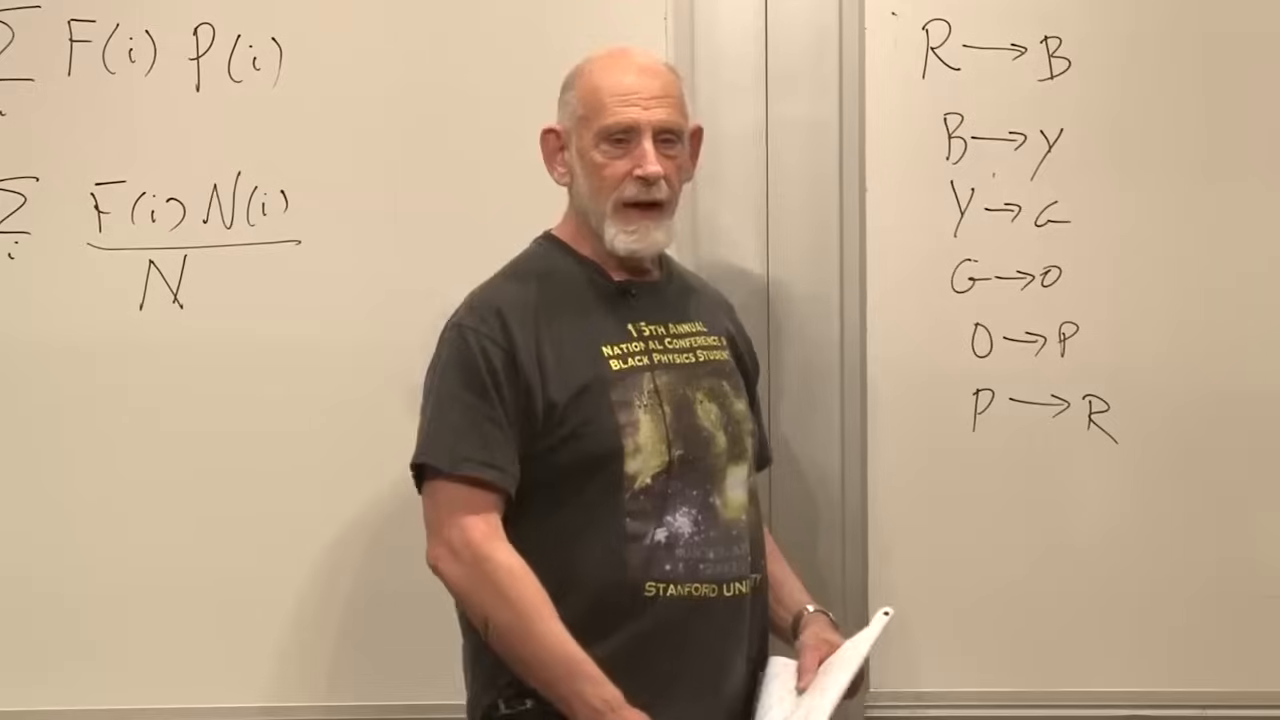
\includegraphics[width=0.92\textwidth]{lecture_01_figure_02.png}
\caption{기댓값 공식은 왼쪽 칠판에 그대로 두고, 결정론적 색상 갱신 규칙 여섯 가지는 오른쪽에 나열했다.}
\lectureframe{00:26:28}
\end{figure}

칠판에 나열된 규칙은 다음과 같이 방향이 있는 순환으로 나타내면 더 명확하다:
\begin{figure}[htbp]
\centering
\begin{tikzpicture}[
  >=Latex,
  state/.style={draw,circle,minimum size=8mm,inner sep=1pt}
]
\node[state] (R) at (90:2.2) {$R$};
\node[state] (B) at (30:2.2) {$B$};
\node[state] (Y) at (-30:2.2) {$Y$};
\node[state] (G) at (-90:2.2) {$G$};
\node[state] (O) at (-150:2.2) {$O$};
\node[state] (P) at (150:2.2) {$P$};
\draw[->] (R) -- (B);
\draw[->] (B) -- (Y);
\draw[->] (Y) -- (G);
\draw[->] (G) -- (O);
\draw[->] (O) -- (P);
\draw[->] (P) -- (R);
\end{tikzpicture}
\caption{여섯 상태로 이루어진 단일 궤도. 한 주기 동안 모든 상태를 한 번씩 방문한다.}
\label{fig:sm1-six-cycle}
\end{figure}

초기 상태를 모르고 시각도 알 수 없는 때에 스냅숏을 찍는다고 하자. 각 단계의 지속 시간이 같으므로 계는 각 색깔 상태에 주기의 6분의 1씩 머문다.
\begin{equation}
 p(R)=p(B)=p(Y)=p(G)=p(O)=p(P)=\frac16.
 \label{eq:sm1-uniform-cycle}
\end{equation}
이 등확률성은 물체의 모양에서 비롯되지 않는다. 각 상태에 머무는 시간이 같은 데서 나온다.

화살표 순서를 바꾸면 미시적 법칙은 달라지지만, 여전히 여섯 상태가 하나의 순환을 이룰 수 있다. 세부적인 순서는 바뀌어도 스냅숏 확률은 \(1/6\)로 유지된다. 각 상태가 주기마다 한 번씩 나타나기 때문이다. 따라서 이 예측에는 출발점이나 세부 순서가 필요하지 않다. 궤도의 구조와 갱신 단계마다 같은 시간이 든다는 사실만 있으면 된다.

\begin{classroomqa}
\classquestion{물체가 대칭이 아닌데도 모든 색깔에 확률 \(1/6\)를 부여하는 것은 어떤 의미에서 정당한가?}
\lecturerresponse{이 확률 배정은 기하학적 대칭성이 아니라 동역학에 근거한다. 여섯 단계 궤도에서 어느 위상에 있는지 모르는 상태로 스냅숏을 찍으면 동일한 시간 간격의 여섯 시간 구간을 표본으로 얻게 된다. 여기서 동등한 것은 물체의 면이 아니라 궤도상의 위치다. 각 상태에 머무는 시간이 서로 다르다면 확률도 서로 달라진다.
\lecturetimestamp{00:27:11--00:29:49}}
\end{classroomqa}

\section{분리된 순환과 보존량}

결정론적 법칙이 모든 상태를 하나의 궤도에 놓을 필요는 없다. 서로 연결되지 않은 두 순환을 생각해 보자.
\begin{equation}
 R\longrightarrow B\longrightarrow G\longrightarrow R,
 \qquad
 P\longrightarrow Y\longrightarrow O\longrightarrow P.
 \label{eq:sm1-two-cycles}
\end{equation}
계가 첫 번째 순환에 있다는 것을 안다면,
\begin{equation}
 \begin{aligned}
 p(R)=p(B)=p(G)&=\frac13,\\
 p(P)=p(Y)=p(O)&=0.
 \end{aligned}
\end{equation}
두 번째 순환에 있다는 것을 알면 이 확률 배정은 반대가 된다.

더 일반적인 경우에는 사전 가중치가 필요하다. 순환을 \(+1\)와 \(-1\)로 표시하고, 각각의 확률을 \(p_+\)와 \(p_-\)라 하자. 이때
\begin{equation}
 p_++p_-=1.
\end{equation}
그러면 다음과 같다.
\begin{align}
 p(R)=p(B)=p(G)&=\frac{p_+}{3},\\
 p(P)=p(Y)=p(O)&=\frac{p_-}{3}.
 \label{eq:sm1-sector-weights}
\end{align}
계수 \(1/3\)는 순환 안에서의 운동으로 정해진다. 반면 \(p_+\)와 \(p_-\)는 그렇지 않다. 이 값들은 다른 실험이나 초기 섹터를 선택하는 다른 계처럼 추가적인 지식에서 얻어야 한다.

표지 \(+1\)와 \(-1\)는 보존량을 정의한다. 계가 한 순환에서 시작하면 갱신 법칙은 그 계를 다른 순환으로 옮기지 않는다. 이 양을 에너지라고 부를 수도 있고, \emph{질크} 같은 임시 이름을 붙일 수도 있다. 이름은 부차적이다. 보존된다는 것은 동역학이 넘나들 수 없는 영역들로 상태공간이 나뉜다는 뜻이다.

순환마다 상태 수가 같을 필요는 없다. 네 상태 궤도와 두 상태 궤도도 두 개의 보존 섹터를 이룬다. 그러면 같은 시간 동안 표본을 취할 때 첫 번째 섹터 안에서는 \(1/4\), 두 번째 섹터 안에서는 \(1/2\)의 확률이 주어지며, 각 확률에는 해당 섹터의 사전 확률을 곱한다. 통계역학은 논리적으로 서로 다른 두 질문에 답해야 한다.
\begin{enumerate}
\item 보존 섹터가 주어졌을 때, 동역학은 그 안의 상태들에 시간을 어떻게 배분하는가?
\item 보존 섹터 자체에는 어떤 확률을 부여해야 하는가?
\end{enumerate}

\begin{classroomqa}
\audiencequestion{보존 섹터 하나 안의 모든 상태에 같은 확률을 부여한다고 가정하는 건가요?}
\lecturerresponse{여기서 제시한 이산 장난감 법칙에서는 그렇다. 각 상태가 같은 시간 간격 동안 지속되고 운동이 결정론적이기 때문이다. 불확실성은 궤도의 초기 위상에 있다. 밀리초 단위로 시간을 재는 검출기로는 마이크로초 단위 갱신을 분해할 수 없지만, 충분히 빠른 스냅숏이라면 포착된 상태를 알아낼 수 있다. 더 일반적인 계에서는 상태별로 머무는 시간이 다를 경우 이를 명시적으로 반영해야 한다.
\lecturetimestamp{00:36:16--00:37:17}}
\end{classroomqa}

\begin{classroomqa}
\audiencequestion{스냅숏을 두 번 찍었을 때 첫 번째 결과로 순환 하나를 알아냈다면, 두 번째 결과에서도 같은 순환이 나와야 하나요?}
\lecturerresponse{그렇다. 바로 그것이 보존의 뜻이다. 측정으로 보존량의 값을 알아내면, 이후 확률은 그 값을 조건으로 삼아 정할 수 있고 다른 섹터에 속한 상태의 확률은 0이 된다.
\lecturetimestamp{00:37:18--00:37:45}}
\end{classroomqa}

\subsection{두 계 사이에서 나뉘는 에너지}

이제 추상적인 표지 대신 에너지를 생각해 보자. 고립된 상자 하나는 닫힌계이므로 보존되는 에너지를 갖는다. 서로 상호작용하지 않는 고립된 상자 두 개에는 각각 따로 보존되는 에너지가 있다. 에너지가 이동할 수 있도록 두 상자를 좁은 통로로 연결하면 각 에너지는 변할 수 있지만 전체 에너지는 일정하게 유지된다.

\begin{figure}[htbp]
\centering
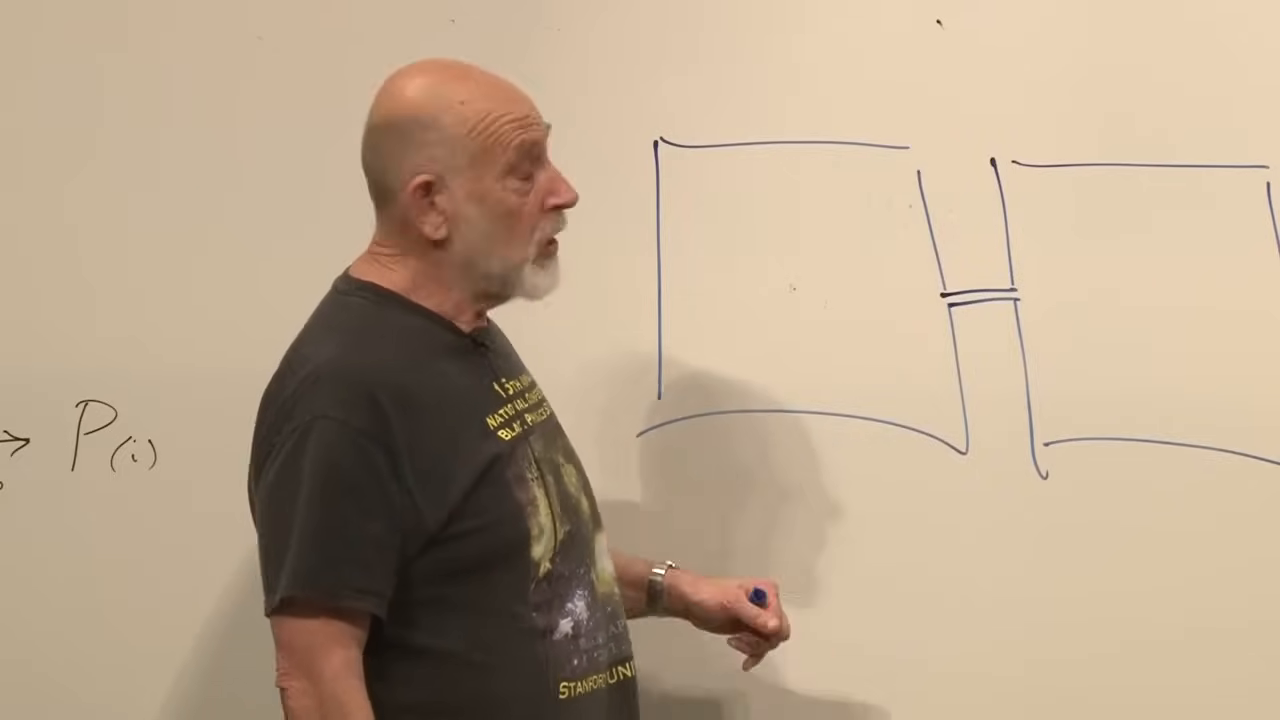
\includegraphics[width=0.92\textwidth]{lecture_01_figure_03.png}
\caption{에너지가 통과할 수 있는 좁은 통로로 연결된 두 부분계.}
\lectureframe{00:39:19}
\end{figure}

\begin{figure}[htbp]
\centering
\begin{tikzpicture}[>=Latex]
\draw[thick,rounded corners=4pt] (-4,1.8) rectangle (-0.7,-1.5);
\draw[thick,rounded corners=4pt] (0.7,1.5) rectangle (4,-1.8);
\draw[thick] (-0.7,0.45) -- (0.7,0.45);
\draw[thick] (-0.7,-0.35) -- (0.7,-0.35);
\draw[<->,very thick] (-0.45,0.05) -- (0.45,0.05);
\node at (-2.35,0.15) {subsystem \(1\)};
\node at (2.35,-0.15) {subsystem \(2\)};
\node[above] at (0,0.5) {energy exchange};
\end{tikzpicture}
\caption{연결을 열면 보존되는 것은 \(E_1+E_2\)뿐이다. 에너지의 분배는 확률 문제로 바뀐다.}
\label{fig:sm1-connected-systems}
\end{figure}

전체 에너지가 주어졌을 때, 부분계 \(1\)의 에너지가 \(E_1\)이고 부분계 \(2\)의 에너지가 나머지인 확률을 물을 수 있다. 같은 크기의 상자라면 평균 에너지도 같아야 하지만, 평균만으로 분포 전체를 알 수는 없다. 따라서 부분계의 확률을 정하는 한 가지 방법은 보존법칙이 필요한 정보를 제공하는 더 큰 닫힌계 안에 그 부분계를 두는 것이다. 이 구성은 통계역학에서 거듭 등장한다.

\section{좋은 법칙, 나쁜 법칙, 그리고 마이너스 제1법칙}

모든 결정론적 갱신 규칙이 근본 법칙으로 허용되는 것은 아니다. 다음 사상을 보자.
\begin{equation}
 \begin{aligned}
 R&\mapsto R,& B&\mapsto R,& Y&\mapsto R,\\
 G&\mapsto R,& O&\mapsto R,& P&\mapsto R.
 \end{aligned}
 \label{eq:sm1-all-to-red}
\end{equation}
이 사상은 미래를 완벽하게 예측한다. 한 단계 뒤에는 상태가 빨간색이 된다. 하지만 반대 방향으로는 문제가 있다. 계가 빨간색이 된 뒤에는 파란색, 노란색, 초록색, 주황색, 보라색 또는 빨간색 자체 중 어느 상태에서 왔는지 알 수 없다.

\begin{figure}[htbp]
\centering
\begin{tikzpicture}[
  >=Latex,
  state/.style={draw,circle,minimum size=8mm,inner sep=1pt}
]
\node[state,fill=red!12] (R) at (0,0) {$R$};
\node[state] (B) at (-3,1.6) {$B$};
\node[state] (Y) at (-3,0) {$Y$};
\node[state] (G) at (-3,-1.6) {$G$};
\node[state] (O) at (3,1.6) {$O$};
\node[state] (P) at (3,-1.6) {$P$};
\draw[->] (B) -- (R);
\draw[->] (Y) -- (R);
\draw[->] (G) -- (R);
\draw[->] (O) -- (R);
\draw[->] (P) -- (R);
\draw[->,loop above] (R) to (R);
\end{tikzpicture}
\caption{다대일 법칙은 다음 상태를 예측하지만, 가능한 과거 상태들 사이의 구별을 지워 버린다.}
\label{fig:sm1-bad-law}
\end{figure}

반면 닫힌 순환은 기록을 보존한다. 경과 시간을 알고 있으면 수천 주기가 지난 뒤에도 상태를 미래나 과거 방향으로 변화시킬 수 있다. 이 법칙은 초기 조건 사이의 차이를 보존한다. Susskind는 이 요구를 \emph{물리학의 마이너스 제1법칙}이라고 부른다. 정보는 근본적으로 사라지지 않는다.

유한한 이산 상태공간에서는 그림으로 나타낸 기준이 간단하다.
\begin{quote}
좋은 법칙에서는 모든 상태에 나가는 화살표가 정확히 하나 있고, 들어오는 화살표도 정확히 하나 있다.
\end{quote}
나가는 화살표는 미래를 정하고, 들어오는 화살표는 과거를 복원한다. 수학적으로 갱신은 상태들의 순열이다.

\subsection{마찰은 겉보기 반례일 뿐}

연속적인 계에 해당하는 정리는 리우빌 정리다. 마찰은 이 정리에 모순되는 듯 보인다. 지우개를 책상 위에서 밀면 어디에서 시작하든 결국 멈춘다. 저항력을 나타내는 개략적인 방정식은 다음과 같다.
\begin{equation}
 m\ddot x=-\gamma\dot x,
 \qquad \gamma>0.
 \label{eq:sm1-drag}
\end{equation}
속도는 지수적으로 감소한다. 봉인된 방에 있는 모든 입자에 적용되는 근본 법칙이 이것뿐이라면, 모든 운동이 사라지고 온도가 0까지 떨어지며 많은 초기 상태가 하나의 최종 상태로 합쳐질 것이다. 에너지 보존은 깨지고, 정보는 사라지며, 무질서도 감소할 것이다. 이는 모든 상태가 빨간색으로 가는 연속계 버전이다.

실제 마찰은 이런 식으로 작용하지 않는다. 지우개는 책상과 지우개 자체, 그리고 주변 환경을 가열한다. 미시적인 위치와 운동량에는 눈에 보이는 운동에서 사라진 구분이 기록된다. 마찰은 관측하지 않은 자유도를 생략한 뒤 부분계에 적용하는 유효 방정식이다. 완전한 닫힌계에 적용되는 근본적인 소산 법칙은 아니다.

\begin{classroomqa}
\classquestion{미분방정식
\(m\ddot x=-\gamma\dot x\)은 무엇을 나타내며, 왜 닫힌계의 근본 법칙이 아닌가요?}
\lecturerresponse{이 방정식은 점성 저항력을 나타낸다. 방정식만 따로 보면 모든 속도를 0으로 이끌며, 이는 초기 온도와 관계없이 기체를 0까지 냉각시킨다. 실제 닫힌계를 기술할 때는 사라진 역학적 에너지와 정보가 미시적 자유도로 옮겨간다. 저항력 방정식은 그런 변수들을 생략한 뒤에만 유효하다.
\lecturetimestamp{00:44:40--00:48:56}}
\end{classroomqa}

\section{점유 상태와 첫 번째 엔트로피}

정보 보존에는 이에 상응하는 확률론적 진술이 있다. 같은 확률을 부여받는 상태가 \(M\)개이고, 전체 상태는 \(N\)개라고 하자.
\begin{equation}
 p_i=
 \begin{cases}
 1/M, & i\text{ in the occupied set},\\
 0, & i\text{ outside it}.
 \end{cases}
 \label{eq:sm1-uniform-occupied}
\end{equation}
정보를 보존하는 갱신은 점유된 상태들을 재배열할 수는 있지만 하나로 합칠 수는 없다. 이후 어느 시점에도 확률이 \(1/M\)인 상태는 \(M\)개 그대로다. 반면 잘못된 사상 \eqref{eq:sm1-all-to-red}은 점유된 여러 상태를 하나로 합칠 수 있다.

수 \(M\)는 무지를 나타낸다. \(M=N\)이면 모든 상태가 가능하고 무지가 최대다. \(M=1\)이면 미시적 상태를 정확히 알고 있다. 따라서 엔트로피를 처음 정의하면 다음과 같다.
\begin{equation}
 S=\log M.
 \label{eq:sm1-entropy-logm}
\end{equation}
그러면 다음을 얻는다.
\begin{equation}
 S_{\max}=\log N,
 \qquad
 S_{\min}=0.
\end{equation}
상태공간이 무한하면 유한한 상한이 없을 수도 있다.

이 전개에서는 온도보다 먼저 엔트로피가 등장하며, 에너지 보존을 정식으로 서술하기도 전에 나온다. 그런 의미에서 엔트로피가 더 원초적이다. 그러나 엔트로피는 역학계 자체만의 성질은 아니다. 엔트로피는 계와 알려진 바를 나타내는 확률분포에 함께 의존한다. 서로 다른 정보를 가진 관측자는 같은 역학계에 서로 다른 엔트로피를 부여할 수 있다.

정확한 미시적 시간발전에서는 점유된 상태들이 재배열될 뿐이므로 이 세분된 엔트로피는 보존된다. 실제로는 시간 측정을 놓치고, 상관관계를 버리며, 엄청나게 많은 변수를 추적하지 못한다. 그러면 확률분포가 더 많은 대안에 걸쳐 퍼지고, 거친 기술에 부여되는 엔트로피가 증가한다. 우리가 쓸 수 있는 기술에서 정보가 사라지더라도 방정식 자체가 정보를 파괴할 필요는 없다.

\begin{classroomqa}
\classquestion{상태가 \(N\)개인 유한한 계에서 가능한 최대 엔트로피는 얼마인가요?}
\lecturerresponse{그 값은 \(\log N\)이며, \(N\)개 상태 모두가 같은 확률일 때 달성된다. 최소 엔트로피는 0이며, 상태 하나의 확률이 1일 때 달성된다. 따라서 엔트로피는 이용 가능한 상태공간뿐 아니라 지식의 상태도 측정한다.
\lecturetimestamp{00:56:46--00:58:19}}
\end{classroomqa}

\section{연속 위상공간에서의 리우빌 흐름}

위치와 운동량이 연속적으로 변하는 입자에서 미시적 상태는 위상공간의 한 점이다. 좌표를 \(q_a\), 그 켤레 운동량을 \(p_a\)라고 쓰자. 입자가 많으면 축도 엄청나게 많다. \(q\)축 하나와 \(p\)축 하나로 그린 2차원 그림은 실제를 대신한 모형일 뿐이다. 각 좌표에 대응하는 운동량이 있으므로 위상공간의 차원은 짝수다.

우리의 지식을 영역 \(\Omega_0\)로 나타낸다고 하자. 확률밀도는 그 영역 안에서 균일하고 바깥에서는 0이다. 예를 들어 모든 입자가 방 안에 있다는 사실을 알면 위치 좌표의 범위가 제한되고, 속도에 상한과 하한을 두면 운동량 좌표의 범위가 제한된다.

해밀토니안 시간 발전은 위상 공간의 각 점을 궤적을 따라 이동시킨다. 서로 가까운 점은 가까운 점으로 이동하고, 점유된 영역은 비압축성 유체의 한 덩어리처럼 흐른다:
\begin{figure}[htbp]
\centering
\begin{tikzpicture}[>=Latex,scale=0.95]
\draw[->] (-4.2,0) -- (4.3,0) node[right] {$q$};
\draw[->] (-3.7,-2.2) -- (-3.7,2.4) node[above] {$p$};
\draw[fill=blue!12,thick]
  (-3.0,-0.5) .. controls (-2.7,1.0) and (-1.3,1.2) .. (-0.9,0.1)
  .. controls (-0.6,-1.0) and (-2.2,-1.4) .. cycle;
\node at (-1.9,0.0) {$\Omega_0$};
\draw[->,very thick] (-0.3,0.2) -- (0.8,0.2);
\draw[fill=orange!15,thick]
  (1.2,-1.1) .. controls (1.5,0.3) and (2.3,1.8) .. (3.2,1.1)
  .. controls (3.6,0.7) and (2.8,-0.4) .. (2.5,-1.5)
  .. controls (2.1,-1.8) and (1.5,-1.6) .. cycle;
\node at (2.35,0.1) {$\Omega_t$};
\end{tikzpicture}
\caption{해밀토니안 흐름은 점유된 위상 공간 영역을 늘이고 비틀 수 있지만, 그 부피는 보존한다.}
\label{fig:sm1-liouville-flow}
\end{figure}

리우빌 정리는 다음과 같이 말한다.
\begin{equation}
 \operatorname{Vol}(\Omega_t)
 =
 \operatorname{Vol}(\Omega_0).
 \label{eq:sm1-liouville-volume}
\end{equation}
초기 밀도가 \(\Omega_0\)에서 균일하면, 시간에 따라 이동한 밀도는 \(\Omega_t\)에서 균일하다. 이는 점유된 이산 상태의 수와 가중치를 보존하는 것에 해당하는 연속적 명제다.

이 정리는 마찰 문제를 기하학적으로도 해결한다. 지우개의 눈에 보이는 운동량만 보면 가능한 상태의 분포가 \(p=0\) 쪽으로 모이는 듯하다. 하지만 전체 위상공간에서는 그 분포가 지우개와 책상 분자들의 위치와 운동량에 걸쳐 퍼진다. 전체 고차원 부피가 일정한 채로 투영은 수축할 수 있다.

\begin{classroomqa}
\classquestion{눈에 보이는 모든 궤적이 정지 상태로 다가간다면 점유된 위상공간 영역은 축 \(p=0\) 위의 한 점으로 붕괴한 건가요?}
\lecturerresponse{줄어든 투영에서만 그렇다. 전체 계에는 책상과 지우개, 주변 환경의 미시적 변수가 들어 있다. 눈에 보이는 운동량 범위가 좁아지는 동안 분포는 숨겨진 방향들로 퍼진다. 리우빌 정리는 불완전한 거시적 변수 집합이 아니라 완전한 닫힌 위상공간에 적용된다.
\lecturetimestamp{01:04:37--01:06:29}}
\end{classroomqa}

\section{마이너스 제1법칙에서 제1법칙까지}

\subsection{영 법칙을 잠시 살펴보기}

첫째 법칙을 진술하기 전에 영 법칙을 먼저 소개하는 것이 유용하다. 아직 열평형을 정의하지 않았으므로, 지금은 이 법칙을 구조에 관한 명제로만 제시한다:
\begin{quote}
계 \(A\)이 계 \(B\)와 열평형에 있고, 계 \(B\)가 계 \(C\)와 열평형에 있다면, 계 \(A\)는 계 \(C\)와 열평형에 있다.
\end{quote}
이 추이성이 나중에 온도의 개념을 가능하게 한다. 지금은 이 점을 잠시 미뤄 둔다.

\subsection{에너지 보존}

닫힌계에 대한 제1법칙은 간단히 다음과 같다.
\begin{equation}
 \frac{dE}{dt}=0.
 \label{eq:sm1-first-law}
\end{equation}
이 간결한 식은 그 힘을 감추고 있다. 에너지는 보존량이며, 에너지라는 말은 뒤에서 더 풍부한 열역학적 의미를 갖게 된다.

닫힌계가 두 부분으로 이루어져 있고 각 부분의 에너지가 가산적이라면,
\begin{equation}
 E=E_1+E_2,
\end{equation}
다음과 같이 쓸 수 있다.
\begin{equation}
 \frac{dE_1}{dt}+\frac{dE_2}{dt}=0,
 \qquad\text{or}\qquad
 \frac{dE_1}{dt}=-\frac{dE_2}{dt}.
 \label{eq:sm1-energy-exchange}
\end{equation}
두 번째 식은 에너지 교환을 명시적으로 드러낸다. 한 부분계가 잃은 에너지는 다른 부분계가 얻는다.

가산성 가정에는 주의가 필요하다. 중력으로 상호작용하는 두 입자에는 각각의 운동에너지가 있지만, 두 입자의 상호작용은 쌍에 속하는 퍼텐셜 에너지를 더한다. 두 물체의 에너지를 합한 값으로 정확히 쓸 수는 없어도 전체 에너지는 보존된다.

열역학에서는 가산적인 근사가 매우 잘 성립하는 경우가 많다. 거시적인 에너지는 부피에 비례하는 반면, 가까이 맞닿은 큰 부분들 사이의 짧은 거리 상호작용 에너지는 주로 접촉 면적에 비례하기 때문이다. 큰 탁자를 여러 블록으로 나누어 보자. 각 블록의 내부 에너지는 부피 효과인 반면, 이웃 블록 사이의 결합은 표면 효과다. 블록이 크면 후자는 상대적으로 작다. 식 \eqref{eq:sm1-first-law}은 닫힌계 전체에 대해 정확하다. 부분계에 적용하는 식 \eqref{eq:sm1-energy-exchange}은 상호작용 에너지가 무시할 만하다고 가정한다.

\begin{classroomqa}
\audiencequestion{정규화 조건 \(\sum_i p_i=1\)도 나열된 결과들이 서로 배타적이라고 가정하나요?}
\lecturerresponse{그렇다. 상태 표지는 대안들이 서로 겹치지 않도록 정의된다. 주사위가 노란색 상태라면 동시에 빨간색 상태일 수 없다. 일상적인 표현에서는 색을 섞어 말할 수 있지만, 확률 계산에 사용하는 상태 분할은 서로 배타적인 대안들로 이루어져야 한다.
\lecturetimestamp{01:12:14--01:12:55}}
\end{classroomqa}

\section{엔트로피로 돌아가기}

이제 강의는 앞서 다루다 만 주제로 명시적으로 돌아간다. 감각적으로 익숙한 온도는 유도되는 물리량이다. 온도를 명확히 정의하려면 엔트로피와 에너지가 먼저 정립되어야 한다.

\subsection{일반적인 확률분포}

특수한 정의 \(S=\log M\)는 \(M\)개 상태가 같은 확률을 갖고 나머지 상태의 확률은 모두 0일 때 적용된다. 일반적인 분포는 직사각형 모양일 필요가 없다. 상태 표지에 따라 가중치가 매끄럽게 변할 수도 있고 불규칙하게 변할 수도 있다.

\begin{figure}[htbp]
\centering
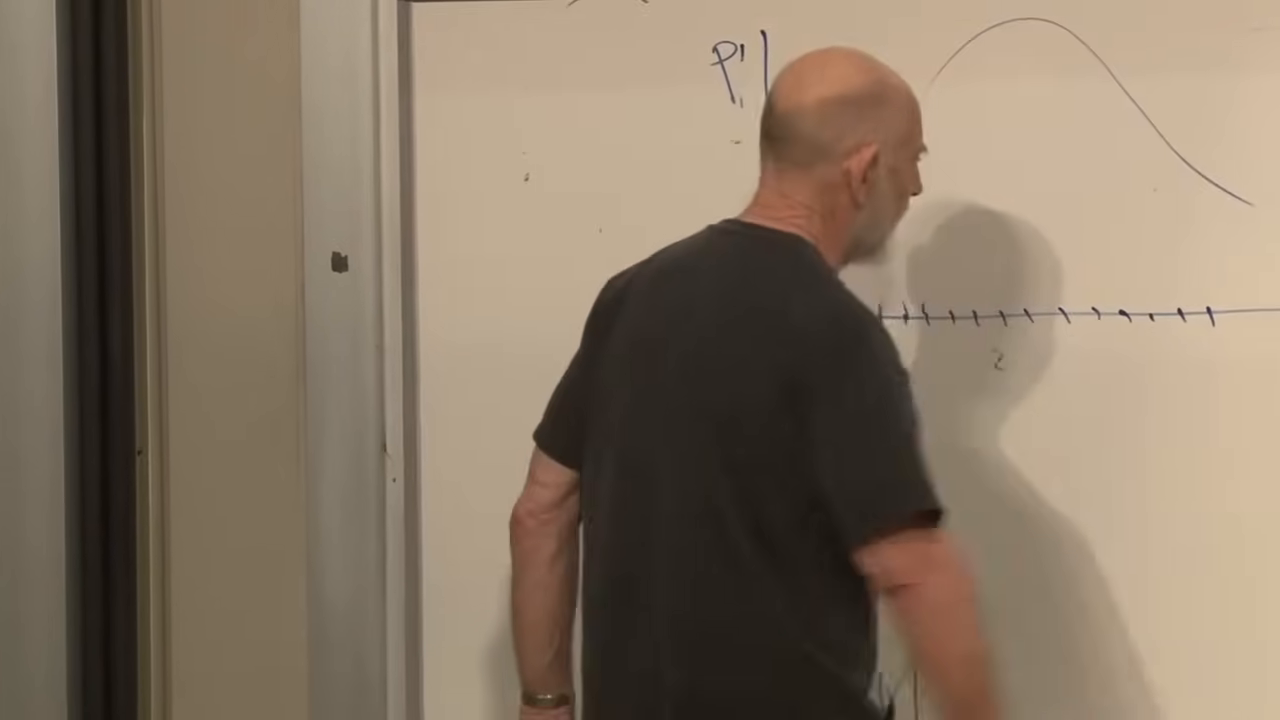
\includegraphics[width=0.92\textwidth]{lecture_01_figure_05.png}
\caption{이산적인 상태 표지 위에 그린 확률분포. 엔트로피를 구하는 데 필요한 특징은 정확한 곡선이 아니라 분포의 퍼짐이다.}
\lectureframe{01:14:40}
\end{figure}

\begin{figure}[htbp]
\centering
\resizebox{\linewidth}{!}{%
\begin{tikzpicture}[>=Latex,scale=0.93]
\draw[->] (-4.2,0) -- (4.4,0) node[right] {state label \(i\)};
\draw[->] (-4,0) -- (-4,3.2) node[above] {$p_i$};
\foreach \x in {-3.6,-3.1,...,3.6}
  \draw (\x,0.08) -- (\x,-0.08);
\draw[very thick]
  plot[smooth] coordinates {
  (-3.7,0.12) (-3.0,0.28) (-2.3,0.72) (-1.6,1.45)
  (-0.9,2.25) (-0.2,2.65) (0.5,2.28) (1.2,1.55)
  (1.9,0.88) (2.7,0.38) (3.5,0.14)};
\draw (-1.8,-0.18) -- (-1.8,-0.5);
\draw (1.8,-0.18) -- (1.8,-0.5);
\draw[<->] (-1.8,-0.46) -- (1.8,-0.46);
\node at (0,-0.82) {effective spread};
\end{tikzpicture}
}
\caption{좁은 분포는 넓은 분포보다 불확실성이 작다. 엔트로피는 분포 전체를 측정해야 한다.}
\label{fig:sm1-probability-spread}
\end{figure}

일반적인 정의는 다음과 같다.
\begin{equation}
 S=-\sum_i p_i\log p_i.
 \label{eq:sm1-shannon-entropy}
\end{equation}
\eqref{eq:sm1-expectation}를 사용하면 다음과 같이 쓸 수 있다.
\begin{equation}
 S=-\langle\log p\rangle.
\end{equation}
\(\log p_i<0\)라는 점을 고려하면 \(0<p_i<1\)일 때 음의 부호가 필요하다.

\subsection{균일분포 결과 되찾기}

일반식이 첫 번째 정의를 재현하는지 확인해야 한다.
비점유 상태에서는 \(p_i=0\)인 반면, \(\log p_i\)는 발산한다. 두 항의 곱은 극한에서 다음과 같이 잘 정의된 값을 갖는다.
\begin{equation}
 \lim_{p\to0^+}p\log p=0.
 \label{eq:sm1-plogp-limit}
\end{equation}
따라서 확률이 0인 상태는 기여하지 않는다.

\begin{classroomqa}
\audiencequestion{\(p_i=0\)이면 이 항은 정말 사라지나요? 영의 로그는 음의 무한대입니다.}
\lecturerresponse{이 항은 \(\lim_{p\to0^+}p\log p\)로 정의되며, 그 값은 영입니다. 인자 \(p\)는 로그가 발산하는 것보다 더 빠르게 영에 가까워집니다. 따라서 확률이 임의로 작아지는 상태들은 임의로 작은 기여를 하고, 정확히 불가능한 상태는 전혀 기여하지 않습니다.
\lecturetimestamp{01:18:27--01:19:46}}
\end{classroomqa}

점유된 \(M\)개의 상태 각각에 대해 \(p_i=1/M\)이다. 따라서
\begin{align}
 S
 &=-\sum_{\mathrm{occupied}\ i}
 \frac1M\log\!\left(\frac1M\right)\\
 &=-M\frac1M\log\!\left(\frac1M\right)\\
 &=-\log\!\left(\frac1M\right)
 =\log M.
 \label{eq:sm1-entropy-check}
\end{align}
일반식은 특수한 경우의 식과 정확히 일치한다. 분포가 넓게 퍼져 있으면 더 많은 대안에 상당한 확률이 부여되므로 엔트로피가 더 크고, 분포가 좁으면 엔트로피가 더 작다.

\begin{figure}[htbp]
\centering
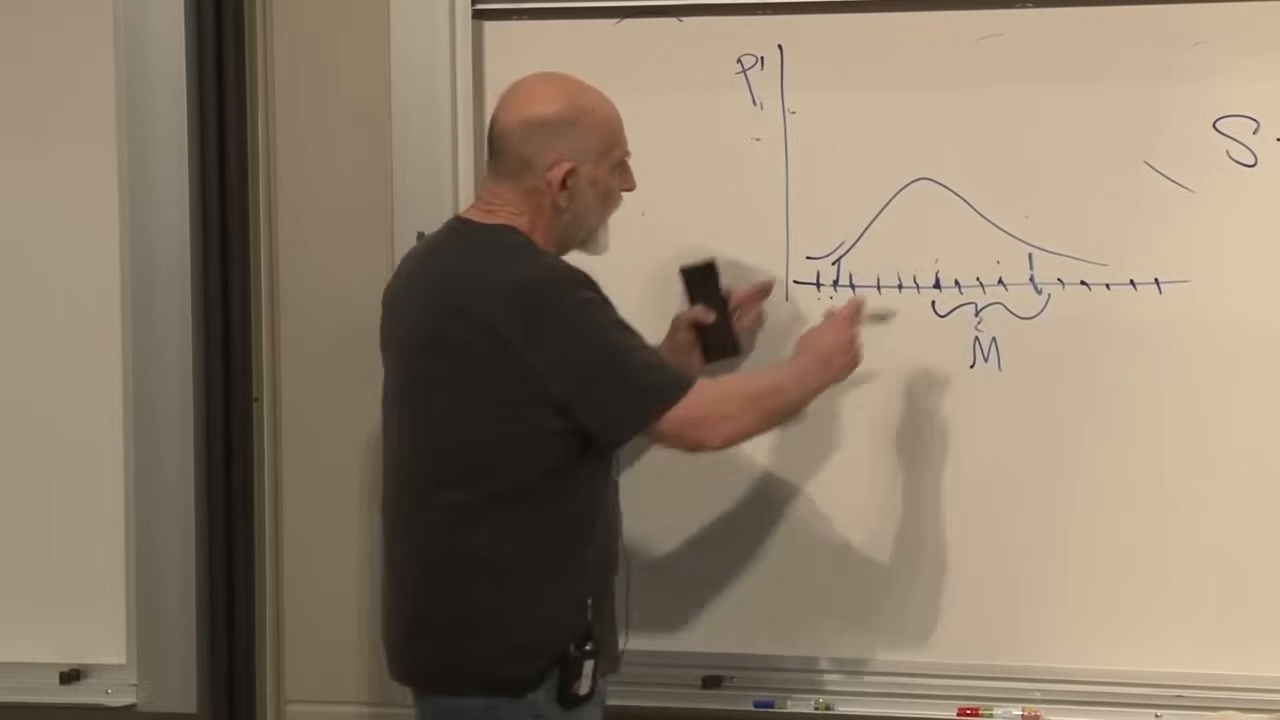
\includegraphics[width=0.92\textwidth]{lecture_01_figure_06.png}
\caption{표시된 폭 \(M\)은 유의미한 확률들의 분포 폭과 엔트로피 사이의 관계를 강조한다.}
\lectureframe{01:16:42}
\end{figure}

엔트로피는 상태 공간 위의 확률분포에 속한다. 한 미시상태의 에너지나 운동량 같은 단순한 관측량이 아니다. 정확한 상태는 그 상태에 집중된 확률분포로 나타낼 수 있으며, 이 경우 엔트로피는 0이다. 그러나 지식의 상태가 달라지면 엔트로피도 달라진다.

\section{동전, 비트, 명시적 계수}

동전의 개수를 \(n\)라고 하자. 미시적 배열의 수는
\begin{equation}
 N=2^n.
 \label{eq:sm1-coin-state-count}
\end{equation}
동전에 대해 아무것도 모른다면 \(2^n\)개의 배열이 모두 같은 확률을 가지며,
\begin{equation}
 S_{\max}=\log(2^n)=n\log2.
 \label{eq:sm1-coin-max-entropy}
\end{equation}
엔트로피는 서로 독립인 동전의 수에 비례해 가산적이다.

밑이 \(2\)인 로그를 사용하면, 두 상태를 가지는 계에 대해 아무것도 모를 때 엔트로피는 1비트다. 자연로그를 사용하면 엔트로피는 \(\log2\)이다. 단위는 관례에 따라 정해지지만, 순서 관계와 가산성은 변하지 않는다.

반대로 동전 하나하나의 상태를 모두 알고 있다면, 정확히 하나의 배열만 확률 1을 갖는다.
\begin{equation}
 S=0.
\end{equation}
아는 것이 많을수록 엔트로피는 작아진다.

이제 \(n\)개의 동전 가운데 정확히 하나만 뒷면이고 나머지는 모두 앞면이며, 뒷면이 어느 위치에 있는지는 모른다고 하자. 뒷면의 위치가 달라지는 \(n\)개의 배열이 같은 확률을 가지므로,
\begin{equation}
 S=\log n.
 \label{eq:sm1-one-tail-entropy}
\end{equation}
이는 일반적으로 \(\log2\)의 정수배가 아니다. 비트는 편리한 단위이지, 모든 엔트로피가 정수 비트 단위로만 나타난다는 뜻은 아니다.

\begin{classroomqa}
\audiencequestion{\(\log2\)는 동전마다 가능한 상태가 두 가지라서 나오는 것뿐인가? 원소의 상태가 세 가지라면 \(\log3\)이 되는가?}
\lecturerresponse{그렇다. \(k\)개의 가능한 상태를 가진 원소의 상태를 균일하게 모르는 경우 그 원소의 기여분은 \(\log k\)이다. 컴퓨터에서 이진 스위치가 특히 편리한 이유는 물리적 스위치가 두 안정 상태를 자연스럽게 구현하고, 2가 자명하지 않은 가장 작은 정수이기 때문이다.
\lecturetimestamp{01:29:55--01:30:48}}
\end{classroomqa}

\begin{classroomqa}
\audiencequestion{로그의 밑은 무엇인가?}
\lecturerresponse{이 물리학 공식에서 \(\log\)는 자연로그를 뜻한다. 정보 이론에서는 흔히 밑이 \(2\)인 로그를 사용해 엔트로피를 비트 단위로 직접 나타낸다. 밑을 바꾸면 모든 엔트로피에 동일한 변환 계수가 곱해질 뿐, 물리적 결론은 달라지지 않는다.
\lecturetimestamp{01:30:49--01:32:06}}
\end{classroomqa}

\section{연속 위상공간의 엔트로피}

고전 위상공간 \(\Gamma\)으로 돌아가자. 확률밀도가 부피 \(V_\Gamma\)인 영역에서 균일하고 바깥에서는 0이라면, 확률이 같은 \(M\)개의 상태를 세는 것에 해당하는 식은 다음과 같다.
\begin{equation}
 S=\log\!\left(\frac{V_\Gamma}{V_0}\right).
 \label{eq:sm1-continuous-uniform}
\end{equation}
여기서 \(V_\Gamma\)는 좌표와 운동량으로 이루어진 고차원 전체 공간의 부피이지, 보통의 공간 부피가 아니다. 고정된 부피 \(V_0\)는 로그의 진수를 무차원으로 만드는 기준 위상공간 셀이다. \(V_0=1\)로 놓으면 칠판에서 사용한 약식 표기 \(S=\log V_\Gamma\)을 얻는다.

일반적인 확률밀도 \(P(q,p)\)의 경우, 이산합은 위상공간 적분으로 바뀐다. 정규화 조건은
\begin{equation}
 \int_\Gamma d\Gamma\,P(q,p)=1,
 \label{eq:sm1-continuous-normalization}
\end{equation}
이며 엔트로피는
\begin{equation}
 S=-\int_\Gamma d\Gamma\,
 P(q,p)\log\!\bigl[P(q,p)V_0\bigr].
 \label{eq:sm1-continuous-entropy}
\end{equation}
이다. 밀도는 위상공간 셀당 확률이다. 개념적으로 \eqref{eq:sm1-continuous-entropy}는 여전히 확률분포가 얼마나 넓게 퍼져 있는지를 나타낸다. 균일한 덩어리 분포의 경우에는 점유 부피를 기준 셀 단위로 나타낸 값의 로그가 된다. 이 고정된 셀을 바꾸면 모든 연속 엔트로피가 같은 가산 상수만큼 이동하므로 엔트로피 차이는 변하지 않는다.

\begin{classroomqa}
\audiencequestion{좌표 기호가 \(x\)에서 \(q\)로 바뀐 이유는 무엇인가?}
\lecturerresponse{물리적 변화는 없다. 고전역학에서는 좌표에 \(x\) 또는 \(q\)를, 켤레 운동량에 \(p\)를 흔히 사용한다. 표기법을 바꾼 것은 단순한 실수였으며 위상공간 구성은 동일하다.
\lecturetimestamp{01:37:10--01:37:39}}
\end{classroomqa}

온도와 볼츠만 분포는 의도적으로 뒤로 미루었다. 다음 과제는 열평형을 정의한 뒤 그에 해당하는 확률분포를 찾는 것이다.

\section{상관관계, 가산성, 정보에 관한 질문}

\subsection{상관관계란 한 측정이 다른 분포를 바꾼다는 뜻이다}

서로 독립인 동전에 대해 아무것도 모른다면 모든 배열에 같은 확률을 부여한다. 이때 동전 하나를 측정해도 다른 동전에 관해서는 아무것도 알 수 없다. 다른 동전들의 분포는 변하지 않는다.

뒷면이 하나인 앙상블은 다르다. 측정한 동전이 뒷면이면 나머지 동전은 모두 확실히 앞면이다. 측정한 동전이 앞면이면 유일한 뒷면은 나머지 \(n-1\)개의 동전 가운데 있어야 하므로, 남은 각 위치에 대한 조건부 확률은
\begin{equation}
\begin{aligned}
 p(&\text{tail at a specified remaining position}\\
   &\mid\text{measured head})=\frac{1}{n-1}.
\end{aligned}
 \label{eq:sm1-conditional-tail}
\end{equation}
이다. 이것이 상관관계다. 한 변수에 대해 알게 되면 다른 변수에 부여하는 확률분포가 달라진다.

\begin{classroomqa}
\audiencequestion{엔트로피 예시에서 동전들의 독립성을 가정했는가?}
\lecturerresponse{완전히 모르는 상태를 \(2^n\)개의 모든 배열에 같은 확률을 부여하는 것으로 나타낸 경우에만 그렇다. 이 경우 동전 하나를 측정해도 나머지 동전들의 분포는 달라지지 않는다. 뒷면이 하나인 예시는 명시적으로 상관되어 있다. 측정하면 다른 곳에서 가능한 상태에 대한 지식이 갱신된다. 주어진 정보에 따라 사용할 확률분포가 정해진다.
\lecturetimestamp{01:38:43--01:41:58}}
\end{classroomqa}

분리된 궤도 예시도 논리 구조가 같다. 보존되는 \(+1\) 또는 \(-1\) 라벨을 측정하면 이후 모든 상태는 하나의 섹터로 제한된다. 보존량에 관한 정보로 조건을 걸면 허용되는 분포가 달라진다.

상관관계가 없는 계들의 엔트로피는 가산적이다. 만약
\begin{equation}
 p_{ij}=p_i^{(A)}p_j^{(B)},
\end{equation}
이라면
\begin{align}
 S_{AB}
 &=-\sum_{i,j}p_i^{(A)}p_j^{(B)}
 \log\!\left[p_i^{(A)}p_j^{(B)}\right]\\
 &=S_A+S_B.
 \label{eq:sm1-entropy-additivity}
\end{align}
이다. 상관관계가 있으면 이 인수분해가 성립하지 않으며 두 계의 독립적인 불확실성은 줄어든다.

연습 삼아, 위 상태일 때 각 이웃 변수가 아래 상태일 확률이 사분의 삼이 되는 이진 변수들의 열을 생각해 보자. 한 위치를 측정하면 인접한 위치에 대해 아는 것이 곧바로 달라진다. 이 분포에는 상관관계가 있으므로, 상관관계를 고려하지 않고 각 위치 하나씩의 엔트로피를 더해서는 전체 엔트로피를 구할 수 없다.

\subsection{볼츠만, 섀넌, 양자 불확정성}

\begin{classroomqa}
\audiencequestion{열역학에서 더 오래전부터 쓰인 엔트로피는 섀넌의 정보 이론적 엔트로피와 어떤 관계인가?}
\lecturerresponse{두 경우에 같은 함수꼴이 나타난다.
\(-\sum_i p_i\log p_i\)섀넌은 흔히 밑이 \(2\)인 로그를 사용했고, 물리학자들은 대개 자연로그를 사용한다. 엔트로피를 열역학적 단위로 나타낼 때는 볼츠만 상수를 다시 곱한다. 수학적 차이는 고정된 변환 계수뿐이지만, 확률을 정하는 물리적 질문은 서로 크게 다를 수 있다.
\lecturetimestamp{01:44:05--01:46:06}}
\end{classroomqa}

미시상태들의 확률이 모두 같을 때 열역학 공식은 흔히 다음과 같이 쓴다.
\begin{equation}
 S_{\mathrm{thermo}}=k_{\mathrm B}\log W,
 \label{eq:sm1-boltzmann-formula}
\end{equation}
여기서 \(W\)는 접근 가능한 미시상태의 수다. \(k_{\mathrm B}=1\)인 단위계에서는 이 식이 정확히 \(S=\log W\)이다. 볼츠만 상수는 온도 단위와 에너지 단위 사이를 변환하며, 온도의 자연스러운 미시적 척도는 에너지다.

\begin{classroomqa}
\audiencequestion{이 엔트로피는 하이젠베르크의 불확정성 원리를 다른 방식으로 표현한 것인가?}
\lecturerresponse{아니다. 여기서 다루는 엔트로피는 가능한 상태들에 대한 확률분포의 불확실성을 측정한다. 양자역학의 언어로는 혼합 상태의 불확실성이지, 순수 상태에서도 남을 수 있는 본질적인 측정 불확실성이 아니다. 두 개념을 구별해야 한다.
\lecturetimestamp{01:46:07--01:47:31}}
\end{classroomqa}

\section{확립된 내용}

출발점은 법칙의 무작위성이 아니었다. 초기 상태에 대한 지식이 불완전하면 결정론적 동역학만으로도 이미 확률이 생긴다. 하나의 궤도에서는 각 상태에 머무는 시간으로 확률 가중치가 정해지고, 서로 분리된 궤도에서는 보존량이 드러나며 각 섹터에 사전 가중치를 부여해야 한다. 허용되는 미시 법칙은 구별되는 상태들을 보존한다. 유한 상태공간에서는 각 상태로 들어오는 화살표와 나가는 화살표가 각각 하나씩 있다는 뜻이며, 연속역학에서는 이를 리우빌 정리로 나타낸다.

이 구조에서 먼저 다음 식이 나온다.
\begin{equation}
 S=\log M
\end{equation}
확률이 같은 점유 상태 \(M\)개에 대해 성립하며, 이어서
\begin{equation}
 S=-\sum_i p_i\log p_i,
\end{equation}
가 나오고, 마지막으로 그 위상공간 적분식에 이른다. 엔트로피는 확률분포, 따라서 지식의 상태를 기록한다. 실용적인 거친 분해능의 기술이 정보를 놓치더라도 미시 법칙은 세분된 정보를 보존한다.

에너지 보존은 첫 번째 법칙을 주며, 부분계 에너지의 가산성에는 상호작용 에너지가 무시할 수 있어야 한다. 엔트로피의 가산성에도 이에 대응하는 조건이 있다. 부분계들의 확률은 서로 상관되어 있지 않아야 한다. 이 두 종류의 가산성을 바탕으로 다음 단계에서는 열평형, 온도, 볼츠만 분포를 통해 에너지와 확률을 연결한다.